% $Id$

The NUOPC generic components are implemented as a {\em collection} of Fortran modules. Each module implements a single, well specified set of standard {\tt ESMF\_GridComp} or {\tt ESMF\_CplComp} methods. The nomenclature of the generic component modules starts with the {\tt NUOPC\_} prefix and continues with the kind: {\tt Driver}, {\tt Model}, {\tt Mediator}, or {\tt Connector}. The four kinds of generic components implemented by the NUOPC Layer are:

\begin{itemize}

\item {\tt NUOPC\_Driver} - A generic driver component. It implements a child component harness, made of State and Component objects, that follows the NUOPC Common Model Architecture. It is specialized by plugging {\tt Model}, {\tt Mediator}, and {\tt Connector} components into the harness. {\tt Driver} components can be plugged into the harness to construct component hierarchies. The generic {\tt Driver} initializes its child components according to a standard Initialization Phase Definition, and drives their Run() methods according a customizable run sequence.

\item {\tt NUOPC\_Model} - A generic model component that wraps a model code so it is suitable to be plugged into a generic {\tt Driver} component.

\item {\tt NUOPC\_Mediator} - A generic mediator component that wraps custom coupling code (flux calculations, averaging, etc.) so it is suitable to be plugged into a generic {\tt Driver} component.

\item {\tt NUOPC\_Connector} - A generic component that implements Field matching based on metadata and executes simple transforms (Regrid and Redist). It can be plugged into a generic {\tt Driver} component.

\end{itemize}

The user code accesses the desired generic component(s) by including a {\tt use} line for each one. Each generic component defines a small set of public names that are made available to the user code through the {\tt use} statement. At a minimum the {\tt SetServices} method is made public. Some of the generic components define additional public routines and labels as part of their user interface. It is recommended to rename entries of an imported generic component module, such as {\tt SetServices}, in the local scope as part of the {\tt use} association to prevent potential name clashes.

\begin{verbatim}
  use NUOPC_<GenericComp>, &
    <GenericComp>SS      => SetServices
\end{verbatim}

A generic component is used by user code to implement a specialized version of the generic component. The user component derives from the generic component code by implementing its own public {\tt SetServices} routine that calls into the generic {\tt SetServices} routine via the {\tt NUOPC\_CompDerive()} method.
Typically this should be the first call made before doing anything else. It is through this mechanism that the deriving component {\em inherits} functionality that is implemented in the generic component. The example below shows how a specific {\em model} component is implemented, deriving from the generic {\tt NUOPC\_Model}:

\begin{verbatim}
  use NUOPC_Model, &
    modelSS => SetServices

  subroutine SetServices(model, rc)
    type(ESMF_GridComp)  :: model
    integer, intent(out) :: rc

    ! derive from NUOPC_Model
    call NUOPC_CompDerive(model, modelSS, rc=rc)

    ! specialize model
    !... calls to NUOPC_CompSpecialize() here
    
  end subroutine
\end{verbatim}

\subsubsection{Component Specialization}

After the call to {\tt NUOPC\_CompDerive()} in a component's {\tt SetServices()} method, the component is connected to all of the generic code provided by NUOPC for the respective component kind. In order to function properly, e.g. as an atmosphere model, ocean model, driver, etc., the component must be {\em specialized}.

The {\tt NUOPC\_CompSpecialize()} method is used to link specific user provided routines to pre-defined NUOPC specialization points. The labels of the pre-defined specialization points are use associated named constants made available by the respective generic component module. The naming of all pre-defined specialization labels starts with the {\tt label\_} prefix, and is followed by a short intent of the specialization. E.g. {\tt label\_Advertise} refers to the specialization point responsible for advertising Fields in the import- and exportStates of the component.

There are pre-defined specialization labels for Initialize, Run, and Finalize phases. Section \ref{PhaseMaps} discusses the semantic labeling of Initialize phases in greater detail. Lists of {\em all} pre-defined specialization labels (Initialize, Run, and Finalize) for each of the generic NUOPC component kinds are provided at the beginning of the respective API sections. (Driver: \ref{NUOPC_Driver}, Model: \ref{NUOPC_Model}, Mediator: \ref{NUOPC_Mediator}, Connector: \ref{NUOPC_Connector})

The following code snippet shows a full specialization of {\tt NUOPC\_Model}, using three specialization labels:

\begin{verbatim}
  use NUOPC_Model, &
    modelSS => SetServices

  subroutine SetServices(model, rc)
    type(ESMF_GridComp)  :: model
    integer, intent(out) :: rc

    rc = ESMF_SUCCESS

    ! derive from NUOPC_Model
    call NUOPC_CompDerive(model, modelSS, rc=rc)
    if (ESMF_LogFoundError(rcToCheck=rc, msg=ESMF_LOGERR_PASSTHRU, &
      line=__LINE__, &
      file=__FILE__)) &
      return  ! bail out

    ! specialize model
    call NUOPC_CompSpecialize(model, specLabel=label_Advertise, &
      specRoutine=Advertise, rc=rc)
    if (ESMF_LogFoundError(rcToCheck=rc, msg=ESMF_LOGERR_PASSTHRU, &
      line=__LINE__, &
      file=__FILE__)) &
      return  ! bail out
    call NUOPC_CompSpecialize(model, specLabel=label_RealizeProvided, &
      specRoutine=Realize, rc=rc)
    if (ESMF_LogFoundError(rcToCheck=rc, msg=ESMF_LOGERR_PASSTHRU, &
      line=__LINE__, &
      file=__FILE__)) &
      return  ! bail out
    call NUOPC_CompSpecialize(model, specLabel=label_Advance, &
      specRoutine=Advance, rc=rc)
    if (ESMF_LogFoundError(rcToCheck=rc, msg=ESMF_LOGERR_PASSTHRU, &
      line=__LINE__, &
      file=__FILE__)) &
      return  ! bail out

  end subroutine
\end{verbatim}

The user implemented specialization routines must follow the NUOPC interface definition.

\begin{verbatim}
  subroutine SpecRoutine(comp, rc)
    type(ESMF_*Comp)      :: comp
    integer, intent(out)  :: rc
  end subroutine
\end{verbatim}

Here {\tt type(ESMF\_*Comp)} either corresponds to {\tt type(ESMF\_GridComp)} for Models, Mediators, and Drivers, or {\tt type(ESMF\_CplComp)} for Connectors.

\subsubsection{Partial Specialization}

Components that are derived from a generic component may choose to only specialize certain aspects, leaving other aspects unspecified. This allows a hierarchy of generic components to be implemented with a high degree of code re-use. The variable level of specialization supports the very differing user needs. Figure \ref{fig:NUOPCGenericComp} depicts the inheritance structure of the standard generic components implemented by the NUOPC Layer. There are two trees, one is rooted in {\tt ESMF\_GridComp}, while the other is rooted in {\tt ESMF\_CplComp}.

\begin{figure}[h]
\begin{center}
\vspace{.5in}
\scalebox{0.6}{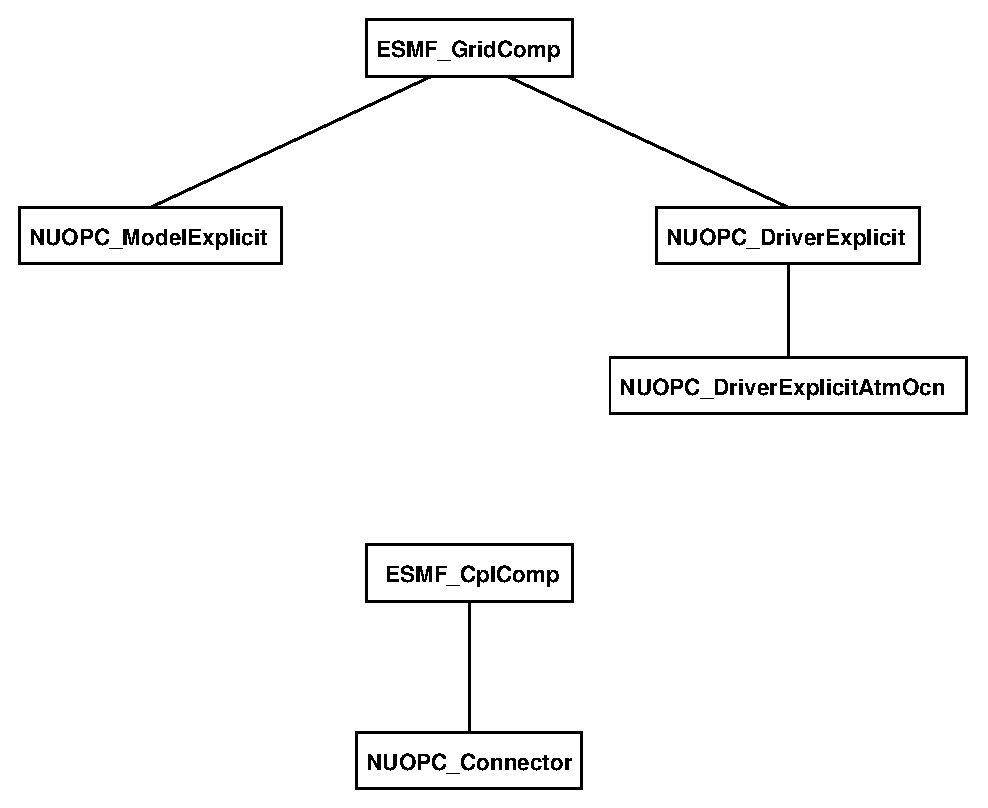
\includegraphics{NUOPC_GC}}
\end{center}
\caption{The NUOPC Generic Component inheritance structure. The tree on the left is rooted in {\tt ESMF\_GridComp}, while the tree on the right is rooted in {\tt ESMF\_CplComp}. The ESMF data types are shown in green. The four main NUOPC Generic Component kinds are shown in dark blue boxes. The yellow box shows a partial specialization in the inheritance tree.}
\label{fig:NUOPCGenericComp}
\end{figure}



